\section{Evaluation} \label{sec:evaluation}
%todo put method in here, if it stays small

\subsection{Unbalanced tree search}

We ran UTS-mem on Grappa and the XMT with two different 100M-vertex trees with a geometric distribution numChildren distribution. Figure~\ref{fig:grappa-xmt-uts} shows the performance in terms of number of vertices visited per second versus number of compute nodes. The Grappa results are for the best parameter values from a limited search over \flushtimeout~and \asyncforthr~\TODO{want to say this in general at beginning of eval?}. Grappa achieves 3x better performance for 12 nodes. Scaling up, Grappa adds 2Mvert/s/node versus XMT's 850Kvert/s/node.



\TODO{why is XMT getting different results for T1L,T2L; would expect it to be the machine with the most uniform results.}

\TODO{sensitivity study for \asyncforthr parameter, ie caching amount. Although we can take advantage of locality in children array and the XMT cannot, we still win without it}


\begin{figure}[h]
    \begin{center}
        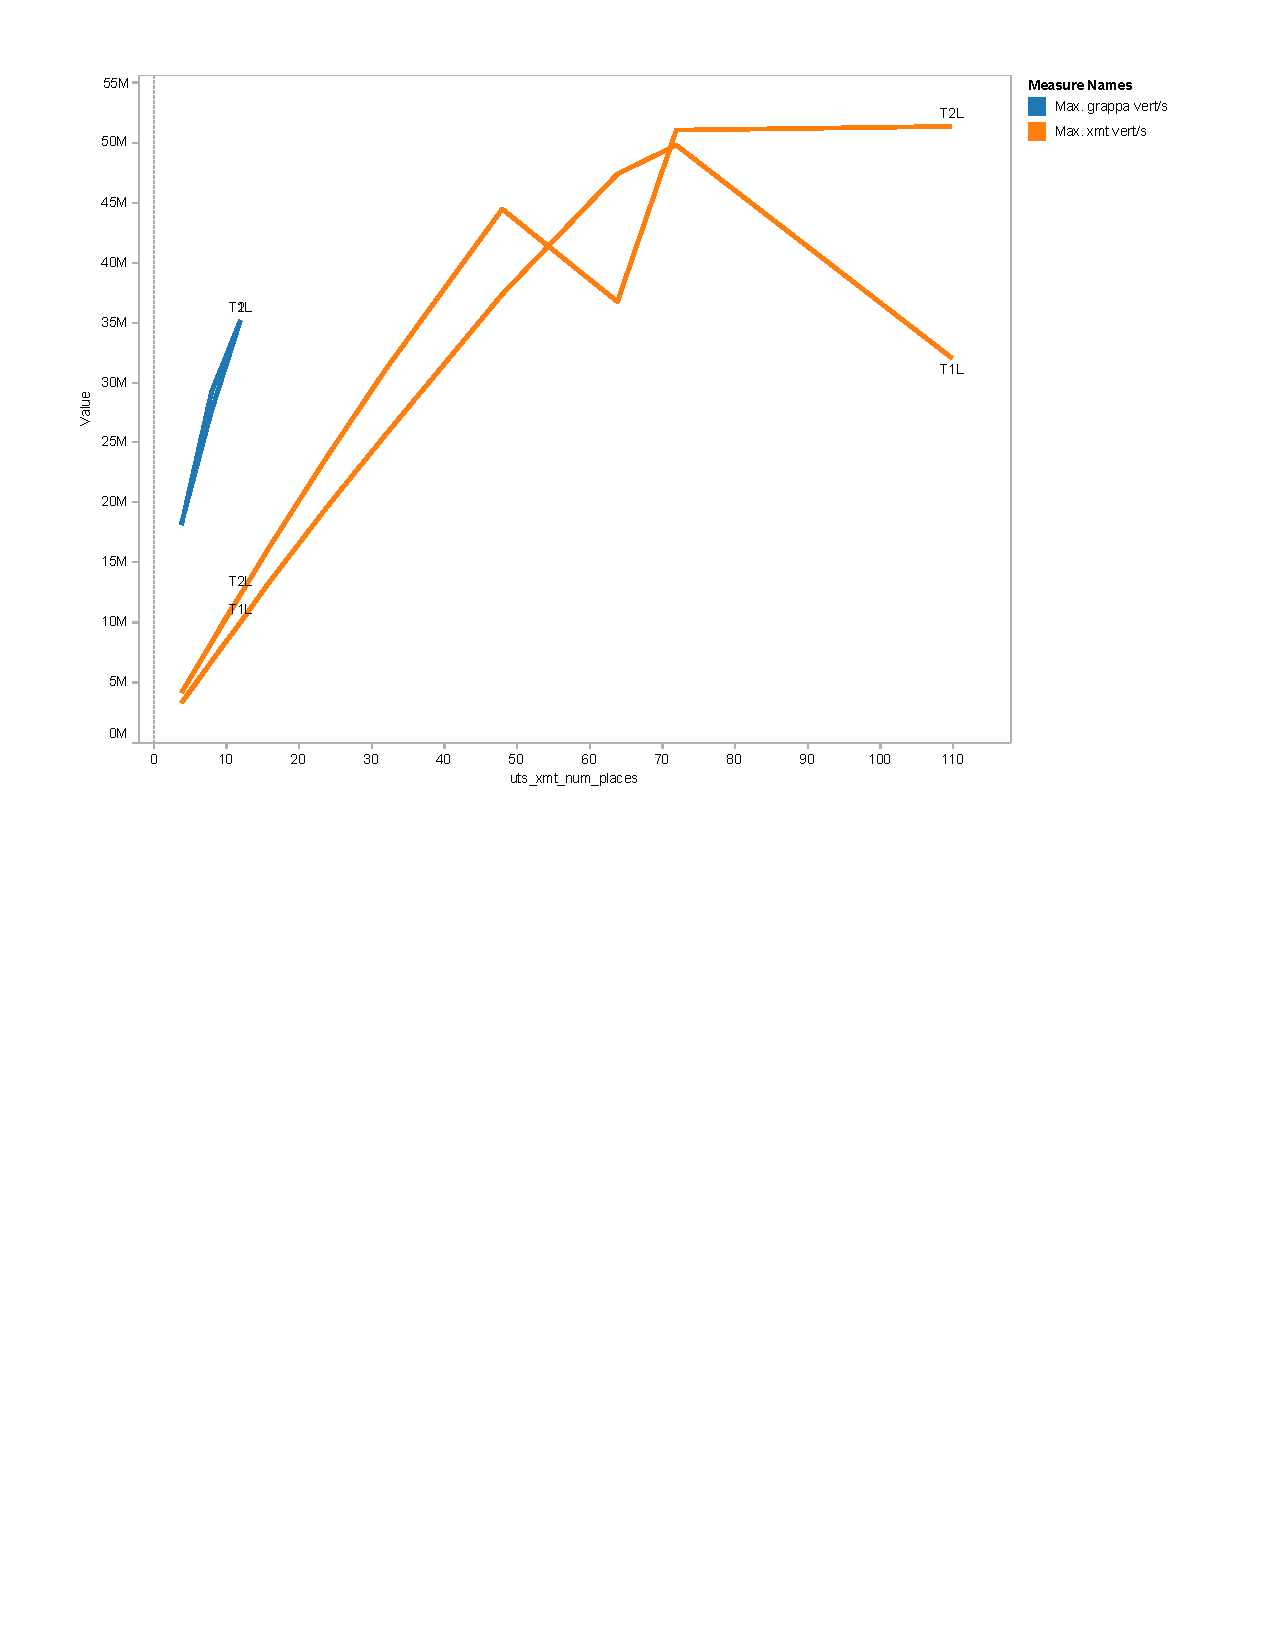
\includegraphics[width=0.5\textwidth]{figs/grappa-xmt-uts.pdf}
    \end{center}
    \caption{describe...}
    \label{fig:grappa-xmt-uts}
\end{figure}


